\documentclass[11pt]{article}
\usepackage[margin=1in]{geometry}
\usepackage{pgfplots}
\usepackage{pgfplotstable}
\usepackage{tikz}
\usepackage{filecontents}
\usepackage{subcaption}
\usepackage{amsmath}
\usepackage{multirow}
\usepackage{pdflscape}
\usepackage{booktabs}

\pgfplotsset{compat=1.17}
\usepgfplotslibrary{statistics}

% Include shared styles
% Define colors for different experiments
\definecolor{exp1}{RGB}{31, 119, 180}
\definecolor{exp2}{RGB}{255, 127, 14}
\definecolor{exp3}{RGB}{44, 160, 44}
\definecolor{exp4}{RGB}{214, 39, 40}
\definecolor{poisson}{RGB}{148, 103, 189}

% Define bar styles for each object (used in bar charts)
\pgfplotsset{
    CuckooBarStyle/.style={fill=exp1!35, draw=exp1!80},
    IcebergBarStyle/.style={fill=exp2!35, draw=exp2!80},
    JunctionBarStyle/.style={fill=exp3!35, draw=exp3!80},
    TPHTBarStyle/.style={fill=exp4!35, draw=exp4!80},
    BlastBarStyle/.style={fill=poisson!35, draw=poisson!80},
    % Macro-based aliases
    htthreeBarStyle/.style={CuckooBarStyle},
    htfourBarStyle/.style={IcebergBarStyle},
    htfiveBarStyle/.style={JunctionBarStyle},
    htoneBarStyle/.style={TPHTBarStyle},
    httwoBarStyle/.style={BlastBarStyle}
} 

% Define line styles for each object (used in line/scatter charts)
\pgfplotsset{
    CuckooLineStyle/.style={color=exp1, mark=o, mark size=2.5pt, thick, smooth},
    IcebergLineStyle/.style={color=exp2, mark=square, mark size=2.5pt, thick, smooth},
    JunctionLineStyle/.style={color=exp3, mark=triangle, mark size=2.5pt, thick, smooth},
    TPHTLineStyle/.style={color=exp4, mark=diamond, mark size=2.5pt, thick, smooth},
    BlastLineStyle/.style={color=poisson, mark=pentagon, mark size=2.5pt, thick, smooth},
    % Macro-based aliases
    htthreeLineStyle/.style={CuckooLineStyle},
    htfourLineStyle/.style={IcebergLineStyle},
    htfiveLineStyle/.style={JunctionLineStyle},
    htoneLineStyle/.style={TPHTLineStyle},
    httwoLineStyle/.style={BlastLineStyle}
}

% Additional utility styles
\pgfplotsset{
    PoissonLineStyle/.style={color=poisson, thick, smooth},
    PoissonFillStyle/.style={color=poisson!20, fill=poisson!20},
    OccScatterStyle/.style={only marks, mark=o, mark size=2.2pt, color=exp1, opacity=0.85}
}

% Backward-compatible aliases for existing macros expecting these names (bar plots)
\pgfplotsset{
    CuckooStyle/.style={CuckooBarStyle},
    IcebergStyle/.style={IcebergBarStyle},
    JunctionStyle/.style={JunctionBarStyle},
    TPHTStyle/.style={TPHTBarStyle},
    BlastStyle/.style={BlastBarStyle},
    % Additional macro-based aliases
    htthreeStyle/.style={CuckooBarStyle},
    htfourStyle/.style={IcebergBarStyle},
    htfiveStyle/.style={JunctionBarStyle},
    htoneStyle/.style={TPHTBarStyle},
    httwoStyle/.style={BlastBarStyle}
}

% Include YCSB helper functions
% Helper function for addplot commands
% #1 = style name, #2 = object_id, #3 = throughput type, #4 = case_id, #5 = entry_id
\newcommand{\addDataPlot}[5]{%
\addplot[#1] table[y expr=\thisrow{#3 (ops/s)}/1000000, restrict expr to domain={\thisrow{entry_id}}{#5:#5}, restrict expr to domain={\thisrow{case_id}}{#4:#4}, restrict expr to domain={\thisrow{object_id}}{#2:#2}]{\data};%
}

% Function to add all 5 plots for standard objects (6,7,15,17,20)
% #1 = case_id, #2 = throughput type, #3 = entry_id
\newcommand{\addAllStandardPlots}[3]{%
\addDataPlot{CuckooStyle}{6}{#2}{#1}{#3}
\addDataPlot{IcebergStyle}{7}{#2}{#1}{#3}
\addDataPlot{JunctionStyle}{15}{#2}{#1}{#3}
\addDataPlot{TPHTStyle}{17}{#2}{#1}{#3}
\addDataPlot{BlastStyle}{20}{#2}{#1}{#3}
}

% Function to add all 5 plots for resizing objects (6,7,15,18,21)
% #1 = case_id, #2 = throughput type, #3 = entry_id
\newcommand{\addAllResizingPlots}[3]{%
\addDataPlot{CuckooStyle}{6}{#2}{#1}{#3}
\addDataPlot{IcebergStyle}{7}{#2}{#1}{#3}
\addDataPlot{JunctionStyle}{15}{#2}{#1}{#3}
\addDataPlot{TPHTStyle}{18}{#2}{#1}{#3}
\addDataPlot{BlastStyle}{21}{#2}{#1}{#3}
}

% Define the 2D dictionary for case_id and entry_id mappings
% When entry_id=0, all case_ids map to "Load"
% When entry_id=1: 17→Run A, 18→Run B, 19→Run C, 20→Run A^-, 21→Run B^-, 22→Run C^-
\def\getlabelname#1#2{%
    \ifnum#2=0%
        Load%
    \else%
        \ifnum#1=17 Run A\fi%
        \ifnum#1=18 Run B\fi%
        \ifnum#1=19 Run C\fi%
        \ifnum#1=20 Run A$^-$\fi%
        \ifnum#1=21 Run B$^-$\fi%
        \ifnum#1=22 Run C$^-$\fi%
    \fi%
}

% Function to generate a subfigure with specified parameters (with y-label) for 1x7 layout
% #1 = case_id (17, 18, 19, 20, 21, 22)
% #2 = caption (Load, Run A, Run B, etc.)
% #3 = throughput type (fill_throughput or run_throughput)
% #4 = entry_id (0 or 1)
\newcommand{\generateSubfigure}[4]{%
\begin{subfigure}[b]{0.14\textwidth}
\centering
\begin{tikzpicture}
\begin{axis}[
    width=3cm,
    height=3.8cm,
    ylabel={Throughput (M/s)},
    ylabel style={at={(ticklabel* cs:1.02)}, anchor=south},
    xlabel={#2},
    ybar,
    bar width=3pt,
    xticklabels={},
    xtick style={draw=none},
    axis lines=box,
    tick align=inside,
    scaled ticks=true,
    tick label style={/pgf/number format/fixed,/pgf/number format/precision=1},
    ymajorgrids=true,
    yminorgrids=true,
    minor tick num=1,
    max space between ticks=35pt,
    try min ticks=5,
    grid style={gray!30},
    ymin=0,
    legend entries = {\htthree, \htfour, \htfive, \htone, \httwo},
    legend cell align = left,
    legend style={draw=none, legend columns=5, /tikz/every even column/.append style={column sep=0.5cm}},
    legend to name={throughput-legend-horizontal}
]
\addAllStandardPlots{#1}{#3}{#4}
\end{axis}
\end{tikzpicture}
\end{subfigure}%
}

% Function to generate a subfigure without y-label (for non-leftmost plots) for 1x7 layout
% #1 = case_id (17, 18, 19, 20, 21, 22)
% #2 = caption (Load, Run A, Run B, etc.)
% #3 = throughput type (fill_throughput or run_throughput)
% #4 = entry_id (0 or 1)
\newcommand{\generateSubfigureNoYLabel}[4]{%
\begin{subfigure}[b]{0.14\textwidth}
\centering
\begin{tikzpicture}
\begin{axis}[
    width=3cm,
    height=3.8cm,
    xlabel={#2},
    ybar,
    bar width=3pt,
    xticklabels={},
    xtick style={draw=none},
    axis lines=box,
    tick align=inside,
    scaled ticks=true,
    tick label style={/pgf/number format/fixed,/pgf/number format/precision=1},
    ymajorgrids=true,
    yminorgrids=true,
    minor tick num=1,
    max space between ticks=35pt,
    try min ticks=5,
    grid style={gray!30},
    ymin=0
]
\addAllStandardPlots{#1}{#3}{#4}
\end{axis}
\end{tikzpicture}
\end{subfigure}%
}

% Function to generate a subfigure for resizing variants for 1x7 layout
% Uses resizable variants: object 18 instead of 17, object 21 instead of 20
\newcommand{\generateSubfigureResizing}[4]{%
\begin{subfigure}[b]{0.14\textwidth}
\centering
\begin{tikzpicture}
\begin{axis}[
    width=3cm,
    height=3.8cm,
    ylabel={Throughput (M/s)},
    ylabel style={at={(ticklabel* cs:1.02)}, anchor=south},
    xlabel={#2},
    ybar,
    bar width=3pt,
    xticklabels={},
    xtick style={draw=none},
    axis lines=box,
    tick align=inside,
    scaled ticks=true,
    tick label style={/pgf/number format/fixed,/pgf/number format/precision=1},
    ymajorgrids=true,
    yminorgrids=true,
    minor tick num=1,
    max space between ticks=35pt,
    try min ticks=5,
    grid style={gray!30},
    ymin=0
]
\addAllResizingPlots{#1}{#3}{#4}
\end{axis}
\end{tikzpicture}
\end{subfigure}%
}

% Function to generate a subfigure for resizing variants without y-label for 1x7 layout
% Uses resizable variants: object 18 instead of 17, object 21 instead of 20
\newcommand{\generateSubfigureResizingNoYLabel}[4]{%
\begin{subfigure}[b]{0.14\textwidth}
\centering
\begin{tikzpicture}
\begin{axis}[
    width=3cm,
    height=3.8cm,
    xlabel={#2},
    ybar,
    bar width=3pt,
    xticklabels={},
    xtick style={draw=none},
    axis lines=box,
    tick align=inside,
    scaled ticks=true,
    tick label style={/pgf/number format/fixed,/pgf/number format/precision=1},
    ymajorgrids=true,
    yminorgrids=true,
    minor tick num=1,
    max space between ticks=35pt,
    try min ticks=5,
    grid style={gray!30},
    ymin=0
]
\addAllResizingPlots{#1}{#3}{#4}
\end{axis}
\end{tikzpicture}
\end{subfigure}%
}

% Legacy functions (kept for backward compatibility but updated for 1x7 layout)
\newcommand{\generateFirstSubfigure}[4]{%
\generateSubfigure{#1}{#2}{#3}{#4}%
}

\newcommand{\generateFirstSubfigureResizing}[4]{%
\generateSubfigureResizing{#1}{#2}{#3}{#4}%
} 

\begin{document}

\title{YCSB Throughput Results and Hash Function Analysis}
\author{}
\date{}
\maketitle

\newcommand{\readdatafiledir}{./}
% Data loading file for TPHT paper
% This file loads all CSV data files from the plots submodule

\pgfplotstableread[col sep=comma, sci]{\readdatafiledir csv/ycsb_results.csv}{\data}
\pgfplotstableread[col sep=comma, sci]{\readdatafiledir csv/occupancy_results.csv}{\occupancydata}
\pgfplotstableread[col sep=comma, sci]{\readdatafiledir csv/throughput_space_eff_results.csv}{\throughputdata}
\pgfplotstableread[col sep=comma, sci]{\readdatafiledir csv/load_factor_support_results.csv}{\loadfactordata}
\pgfplotstableread[col sep=comma, sci]{\readdatafiledir csv/scaling_results.csv}{\scalingdata}
\pgfplotstableread[col sep=comma, sci]{\readdatafiledir csv/occupancy_experimental_box_random.csv}{\occbox}
\pgfplotstableread[col sep=comma, sci]{\readdatafiledir csv/occupancy_poisson.csv}{\occpois}
\pgfplotstableread[col sep=comma, sci]{\readdatafiledir csv/data_size_scaling_results.csv}{\datasizedata}

% New CSV files for intro figure
\pgfplotstableread[col sep=comma, sci]{\readdatafiledir csv/ycsb_intro_summary.csv}{\ycsbintrodata}
\pgfplotstableread[col sep=comma, sci]{\readdatafiledir csv/max_space_efficiency.csv}{\maxspaceeffdata}

% Percentile data
\pgfplotstableread[col sep=comma, sci]{\readdatafiledir csv/percentile_results.csv}{\percentiledata}


% Dictionary reference table
\section{Dictionary Mapping}
\begin{table}[h!]
    \centering
    \begin{tabular}{|c|c|c|}
        \hline
        Case ID & Entry ID & Label     \\
        \hline
        17-22   & 0        & Load      \\
        \hline
        17      & 1        & Run A     \\
        18      & 1        & Run B     \\
        19      & 1        & Run C     \\
        20      & 1        & Run A$^-$ \\
        21      & 1        & Run B$^-$ \\
        22      & 1        & Run C$^-$ \\
        \hline
    \end{tabular}
    \caption{Case ID and Entry ID to Label Mapping}
    \label{tab:dictionary}
\end{table}

% Include YCSB plots

\begin{figure*}[h]
    \centering
    
    \pgfplotslegendfromname{throughput-legend-horizontal}
    
    % Single row: Load, Run A, Run B, Run C, Run A^-, Run B^-, Run C^-
    \generateSubfigure{17}{Load}{fill_throughput}{0}%
    \generateSubfigureNoYLabel{17}{Run A}{run_throughput}{0}%
    \generateSubfigureNoYLabel{18}{Run B}{run_throughput}{0}%
    \generateSubfigureNoYLabel{19}{Run C}{run_throughput}{0}%
    \generateSubfigureNoYLabel{20}{Run A$^-$}{run_throughput}{0}%
    \generateSubfigureNoYLabel{21}{Run B$^-$}{run_throughput}{0}%
    \generateSubfigureNoYLabel{22}{Run C$^-$}{run_throughput}{0}

    \caption{YCSB Throughput Results by Workload Type. Load shows fill throughput from case 17. Run workloads show run throughput from their respective cases (17-22). All data uses entry\_id=0 (resizing disabled).}
    \label{fig:throughput_subfigures}
\end{figure*}


% (Occupancy plots removed)

% Include throughput vs space efficiency plots

% Local helper: add all object plots for a given case_id
% #1 = case_id
\newcommand{\AddAllObjectPlotsForCase}[1]{%
    % \htthree (object_id=6)
    \addplot[CuckooLineStyle] table[
        x=space_efficiency,
        y=throughput_millions,
        restrict expr to domain={\thisrow{object_id}}{6:6},
        restrict expr to domain={\thisrow{case_id}}{#1:#1}
    ] {\throughputdata};

    % \htfour (object_id=7)
    \addplot[IcebergLineStyle] table[
        x=space_efficiency,
        y=throughput_millions,
        restrict expr to domain={\thisrow{object_id}}{7:7},
        restrict expr to domain={\thisrow{case_id}}{#1:#1}
    ] {\throughputdata};

    % \htfive (object_id=15)
    \addplot[JunctionLineStyle] table[
        x=space_efficiency,
        y=throughput_millions,
        restrict expr to domain={\thisrow{object_id}}{15:15},
        restrict expr to domain={\thisrow{case_id}}{#1:#1}
    ] {\throughputdata};

    % \htone (object_id=17)
    \addplot[TPHTLineStyle] table[
        x=space_efficiency,
        y=throughput_millions,
        restrict expr to domain={\thisrow{object_id}}{17:17},
        restrict expr to domain={\thisrow{case_id}}{#1:#1}
    ] {\throughputdata};

    % \httwo (object_id=23)
    \addplot[BlastLineStyle] table[
        x=space_efficiency,
        y=throughput_millions,
        restrict expr to domain={\thisrow{object_id}}{23:23},
        restrict expr to domain={\thisrow{case_id}}{#1:#1}
    ] {\throughputdata};
}

% Common axis style for all space efficiency plots
\pgfplotsset{
    spaceeff axis/.style={
        width=6.2cm,
        height=4cm,
        xlabel={Space Efficiency},
        xmin=-0.05,
        ymin=0,
        grid=major,
        grid style={gray!30},
        tick label style={font=\small},
        label style={font=\small},
        scaled ticks=true,
        tick label style={/pgf/number format/fixed,/pgf/number format/precision=2},
        xtick distance=0.2,
        % ytick distance=10,
        minor tick num=1
    },
    spaceeff axis with ylabel/.style={
        spaceeff axis,
        ylabel={Throughput (M/s)}
    }
}

% Helper: create a subplot for a given case
% #1 = case_id, #2 = position (e.g., [b]{0.45\textwidth}), #3 = extra options for legend
\newcommand{\CreateSpaceEffSubplot}[3]{%
    \begin{subfigure}#2
    \centering
    \begin{tikzpicture}
    \begin{axis}[spaceeff axis, #3]
    \AddAllObjectPlotsForCase{#1}
    \end{axis}
    \end{tikzpicture}
    \caption{Case #1}
    \end{subfigure}%
}

\begin{figure*}[h]
    \centering
    
    % Legend above figures in 1x5 layout
    {\pgfplotslegendfromname{spaceeff-legend}}
    
    % \vspace{0.5cm}
    
    % Case 1 with legend definition and y-label
    \begin{subfigure}[b]{0.35\textwidth}
        \centering
        \begin{tikzpicture}
        \begin{axis}[spaceeff axis with ylabel, legend to name={spaceeff-legend}, legend entries={\htthree, \htfour, \htfive, \htone, \httwo}, legend cell align=left, legend style={draw=none, legend columns=5, /tikz/every even column/.append style={column sep=0.5cm}}]
        \AddAllObjectPlotsForCase{1}
        \end{axis}
        \end{tikzpicture}
        \caption{Insertion}
        \label{fig:throughput_space_efficiency/insertion}
    \end{subfigure}%
    % Case 9 (no y-label)
    \begin{subfigure}[b]{0.32\textwidth}
        \centering
        \begin{tikzpicture}
        \begin{axis}[spaceeff axis]
        \AddAllObjectPlotsForCase{9}
        \end{axis}
        \end{tikzpicture}
        \caption{Positive Query}
        \label{fig:throughput_space_efficiency/positive_query}
    \end{subfigure}%
    % Case 10 (no y-label)
    \begin{subfigure}[b]{0.32\textwidth}
        \centering
        \begin{tikzpicture}
        \begin{axis}[spaceeff axis]
        \AddAllObjectPlotsForCase{10}
        \end{axis}
        \end{tikzpicture}
        \caption{Negative Query}
        \label{fig:throughput_space_efficiency/negative_query}
    \end{subfigure}


    \caption{Throughput-space efficiency tradeoff across insertion and query workloads. Each curve shows how throughput and space efficiency vary with load factor, with rightmost points indicating maximum achievable space efficiency.}
    \label{fig:throughput_space_efficiency_cases}
\end{figure*} 

% Include load factor support plots
\section{Load Factor Support Analysis}

\begin{figure}[p]
    \centering
    \begin{tikzpicture}
        \begin{axis}[
            width=12cm,
            height=8cm,
            xlabel={Bin Size},
            ylabel={Load Factor Support (\%)},
            xmode=log,
            xmin=1,
            xmax=200,
            ymin=0,
            ymax=100,
            grid=major,
            grid style={gray!30},
            legend pos=outer north east,
            legend style={font=\small},
            tick label style={font=\small},
            label style={font=\small},
            title={Load Factor Support vs Bin Size},
            title style={font=\small},
            scaled ticks=true,
            tick label style={/pgf/number format/fixed,/pgf/number format/precision=1}
        ]

        % Plot insertion data (from CSV)
        \addplot[CuckooLineStyle] table[
            x=bin_size,
            y index=3,
            col sep=comma,
            restrict expr to domain={\thisrow{object_id}}{4:4}
        ] {\loadfactordata};
        \addlegendentry{Insertion Only}

        % Plot deletion data (hardcoded)
        \addplot[IcebergLineStyle] coordinates {
            (3,7)
            (7,43)
            (15,71)
            (31,85)
            (63,91)
            (127,95)
        };
        \addlegendentry{With Deletion}

        \end{axis}
    \end{tikzpicture}
    \caption{Load Factor Support vs Bin Size for different hash table implementations. The x-axis shows bin size on a logarithmic scale, while the y-axis shows the maximum supported load factor as a percentage.}
    \label{fig:load_factor_support}
\end{figure} 

% Include scaling plots
% Function to map case numbers to descriptive names
\newcommand{\getCaseName}[1]{%
    \ifnum#1=1 Insertion\fi%
    \ifnum#1=3 Deletion\fi%
    \ifnum#1=6 Positive Query\fi%
    \ifnum#1=7 Negative Query\fi%
}

% Helper macro to plot all objects for a given case
\newcommand{\AddAllObjectPlotsForScaling}[1]{%
    % Cuckoo (object_id=6)
    \addplot[CuckooLineStyle] table[
        x=thread_num,
        y expr=\thisrow{throughput (ops/s)}/1000000,
        restrict expr to domain={\thisrow{case_id}}{#1:#1},
        restrict expr to domain={\thisrow{object_id}}{6:6},
        restrict expr to domain={\thisrow{thread_num}}{0:17}
    ] {\scalingdata};
    
    % Iceberg (object_id=7)
    \addplot[IcebergLineStyle] table[
        x=thread_num,
        y expr=\thisrow{throughput (ops/s)}/1000000,
        restrict expr to domain={\thisrow{case_id}}{#1:#1},
        restrict expr to domain={\thisrow{object_id}}{7:7},
        restrict expr to domain={\thisrow{thread_num}}{0:17}
    ] {\scalingdata};
    
    % Junction (object_id=15)
    \addplot[JunctionLineStyle] table[
        x=thread_num,
        y expr=\thisrow{throughput (ops/s)}/1000000,
        restrict expr to domain={\thisrow{case_id}}{#1:#1},
        restrict expr to domain={\thisrow{object_id}}{15:15},
        restrict expr to domain={\thisrow{thread_num}}{0:17}
    ] {\scalingdata};
    
    % TPHT (object_id=17)
    \addplot[TPHTLineStyle] table[
        x=thread_num,
        y expr=\thisrow{throughput (ops/s)}/1000000,
        restrict expr to domain={\thisrow{case_id}}{#1:#1},
        restrict expr to domain={\thisrow{object_id}}{17:17},
        restrict expr to domain={\thisrow{thread_num}}{0:17}
    ] {\scalingdata};
    
    % Blast (object_id=20)
    \addplot[BlastLineStyle] table[
        x=thread_num,
        y expr=\thisrow{throughput (ops/s)}/1000000,
        restrict expr to domain={\thisrow{case_id}}{#1:#1},
        restrict expr to domain={\thisrow{object_id}}{20:20},
        restrict expr to domain={\thisrow{thread_num}}{0:17}
    ] {\scalingdata};
}


\begin{figure*}[h]
    \centering
    % Display shared legend
    {\pgfplotslegendfromname{spaceeff-legend}}
    % Case 1
    \begin{subfigure}[b]{0.27\textwidth}
        \centering
        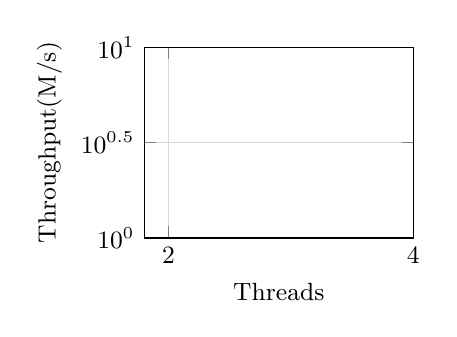
\begin{tikzpicture}
            \begin{axis}[
                    width=5cm,
                    height=4cm,
                    xlabel={Threads},
                    ylabel={Throughput(M/s)},
                    xmode=log,
                    ymode=log,
                    log basis x=2,
                    log basis y=10,
                    xmin=0,
                    xmax=20,
                    ymin=1,
                    ymax=400,
                    xtick={1,2,4,8,16},
                    xticklabels={1,2,4,8,16},
                    ytick={0.1,1,10,100},
                    grid=major,
                    grid style={gray!30},
                    tick label style={font=\small},
                    label style={font=\small},
                    % title={\getCaseName{1}},
                    % title style={font=\small},
                    scaled ticks=true,
                    tick label style={/pgf/number format/fixed,/pgf/number format/precision=1}
                ]

                \AddAllObjectPlotsForScaling{1}

            \end{axis}
        \end{tikzpicture}
        \caption{\getCaseName{1}}
    \end{subfigure}%
    % Case 3
    \begin{subfigure}[b]{0.23\textwidth}
        \centering
        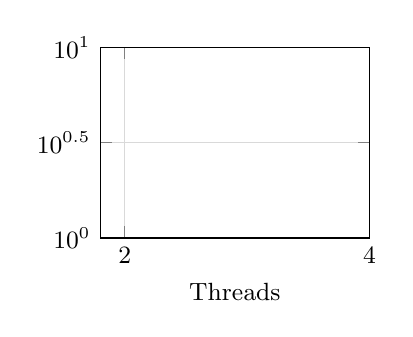
\begin{tikzpicture}
            \begin{axis}[
                    width=5cm,
                    height=4cm,
                    xlabel={Threads},
                    % ylabel={Throughput(M/s)},
                    xmode=log,
                    ymode=log,
                    log basis x=2,
                    log basis y=10,
                    xmin=0,
                    xmax=20,
                    ymin=1,
                    ymax=1000,
                    xtick={1,2,4,8,16},
                    xticklabels={1,2,4,8,16},
                    ytick={0.1,1,10,100,1000},
                    grid=major,
                    grid style={gray!30},
                    tick label style={font=\small},
                    label style={font=\small},
                    % title={\getCaseName{3}},
                    % title style={font=\small},
                    scaled ticks=true,
                    tick label style={/pgf/number format/fixed,/pgf/number format/precision=1}
                ]

                \AddAllObjectPlotsForScaling{3}

            \end{axis}
        \end{tikzpicture}
        \caption{\getCaseName{3}}
    \end{subfigure}%
    % Case 6
    \begin{subfigure}[b]{0.23\textwidth}
        \centering
        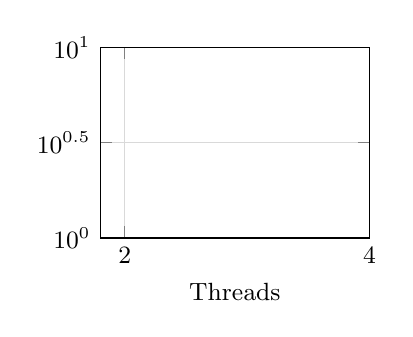
\begin{tikzpicture}
            \begin{axis}[
                    width=5cm,
                    height=4cm,
                    xlabel={Threads},
                    % ylabel={Throughput(M/s)},
                    xmode=log,
                    ymode=log,
                    log basis x=2,
                    log basis y=10,
                    xmin=0,
                    xmax=20,
                    ymin=1,
                    ymax=1000,
                    xtick={1,2,4,8,16},
                    xticklabels={1,2,4,8,16},
                    ytick={0.1,1,10,100,1000},
                    grid=major,
                    grid style={gray!30},
                    tick label style={font=\small},
                    label style={font=\small},
                    % title={\getCaseName{6}},
                    % title style={font=\small},
                    scaled ticks=true,
                    tick label style={/pgf/number format/fixed,/pgf/number format/precision=1}
                ]
                \AddAllObjectPlotsForScaling{6}
            \end{axis}
        \end{tikzpicture}
        \caption{\getCaseName{6}}
    \end{subfigure}%
    % Case 7
    \begin{subfigure}[b]{0.23\textwidth}
        \centering
        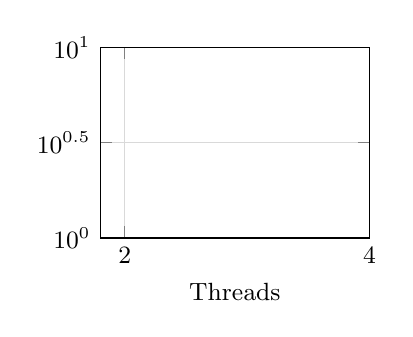
\begin{tikzpicture}
            \begin{axis}[
                    width=5cm,
                    height=4cm,
                    xlabel={Threads},
                    % ylabel={Throughput(M/s)},
                    xmode=log,
                    ymode=log,
                    log basis x=2,
                    log basis y=10,
                    xmin=0,
                    xmax=20,
                    ymin=1,
                    ymax=1000,
                    xtick={1,2,4,8,16},
                    xticklabels={1,2,4,8,16},
                    ytick={0.1,1,10,100,1000},
                    grid=major,
                    grid style={gray!30},
                    tick label style={font=\small},
                    label style={font=\small},
                    % title={\getCaseName{7}},
                    % title style={font=\small},
                    scaled ticks=true,
                    tick label style={/pgf/number format/fixed,/pgf/number format/precision=1}
                ]

                \AddAllObjectPlotsForScaling{7}

            \end{axis}
        \end{tikzpicture}
        \caption{\getCaseName{7}}
    \end{subfigure}%
    \caption{Scaling Analysis for different hash table implementations across various operations. Each subfigure shows throughput scaling with thread count for a specific operation type.}
    \label{fig:scaling_analysis}
\end{figure*}

% Include data size scaling plots
% Helper to map case id to label
\newcommand{\getScalingCaseName}[1]{%
  \ifnum#1=1 Insertion\fi%
  \ifnum#1=3 Deletion\fi%
  \ifnum#1=6 Positive Query\fi%
  \ifnum#1=7 Negative Query\fi%
}

% Helper to add all 5 objects with consistent styles
\newcommand{\AddAllObjectsForDataSize}[1]{%
  % Cuckoo (6)
  \addplot[CuckooLineStyle] table[
    x=table_size,
    y expr=\thisrow{throughput (ops/s)}/1000000,
    restrict expr to domain={\thisrow{case_id}}{#1:#1},
    restrict expr to domain={\thisrow{object_id}}{6:6},
    restrict expr to domain={\thisrow{table_size}}{32768:1000000000}
  ] {\datasizedata};
  % Iceberg (7)
  \addplot[IcebergLineStyle] table[
    x=table_size,
    y expr=\thisrow{throughput (ops/s)}/1000000,
    restrict expr to domain={\thisrow{case_id}}{#1:#1},
    restrict expr to domain={\thisrow{object_id}}{7:7},
    restrict expr to domain={\thisrow{table_size}}{32768:1000000000}
  ] {\datasizedata};
  % Junction (15)
  \addplot[JunctionLineStyle] table[
    x=table_size,
    y expr=\thisrow{throughput (ops/s)}/1000000,
    restrict expr to domain={\thisrow{case_id}}{#1:#1},
    restrict expr to domain={\thisrow{object_id}}{15:15},
    restrict expr to domain={\thisrow{table_size}}{32768:1000000000}
  ] {\datasizedata};
  % TPHT (17)
  \addplot[TPHTLineStyle] table[
    x=table_size,
    y expr=\thisrow{throughput (ops/s)}/1000000,
    restrict expr to domain={\thisrow{case_id}}{#1:#1},
    restrict expr to domain={\thisrow{object_id}}{17:17},
    restrict expr to domain={\thisrow{table_size}}{32768:1000000000}
  ] {\datasizedata};
  % Blast (20)
  \addplot[BlastLineStyle] table[
    x=table_size,
    y expr=\thisrow{throughput (ops/s)}/1000000,
    restrict expr to domain={\thisrow{case_id}}{#1:#1},
    restrict expr to domain={\thisrow{object_id}}{20:20},
    restrict expr to domain={\thisrow{table_size}}{32768:1000000000}
  ] {\datasizedata};
}

% Shared legend (reuse scaling legend styles)
\begin{figure*}[h]
  \centering
  {\pgfplotslegendfromname{spaceeff-legend}}
  % Case 1
  \begin{subfigure}[b]{0.27\textwidth}
    \tiny
    \centering
    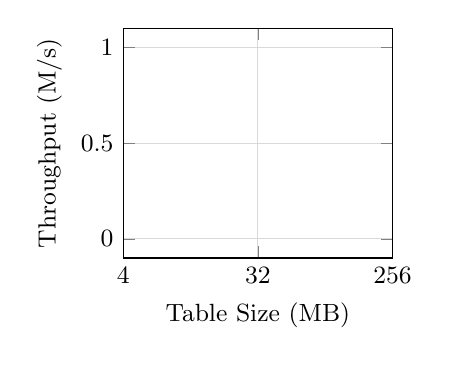
\begin{tikzpicture}
      \begin{axis}[
        width=5cm,
        height=4.5cm,
        xlabel={Table Size (MB)},
        ylabel={Throughput (M/s)},
        xmode=log,
        log basis x=2,
        xmin=131072,
        xmax=268435456,
        xtick={262144,2097152,16777216,134217728},
        xticklabels={4,32,256,2048},
        grid=major,
        grid style={gray!30},
        tick label style={font=\small},
        label style={font=\small},
        scaled ticks=true,
        tick label style={/pgf/number format/fixed,/pgf/number format/precision=1}
      ]
      \AddAllObjectsForDataSize{1}
      \end{axis}
    \end{tikzpicture}
    \caption{\getScalingCaseName{1}}
  \end{subfigure}%
  % Case 3
  \begin{subfigure}[b]{0.24\textwidth}
    \tiny
    \centering
    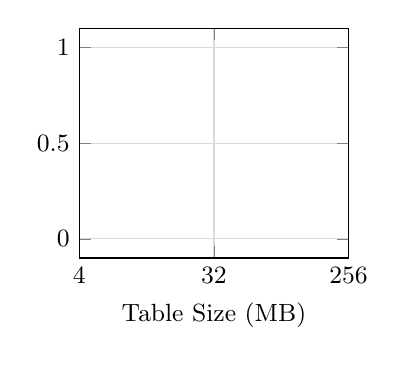
\begin{tikzpicture}
      \begin{axis}[
        width=5cm,
        height=4.5cm,
        xlabel={Table Size (MB)},
        % ylabel={Throughput (M/s)},
        xmode=log,
        log basis x=2,
        xmin=131072,
        xmax=268435456,
        xtick={262144,2097152,16777216,134217728},
        xticklabels={4,32,256,2048},
        grid=major,
        grid style={gray!30},
        tick label style={font=\small},
        label style={font=\small},
        scaled ticks=true,
        tick label style={/pgf/number format/fixed,/pgf/number format/precision=1}
      ]
      \AddAllObjectsForDataSize{3}
      \end{axis}
    \end{tikzpicture}
    \caption{\getScalingCaseName{3}}
  \end{subfigure}%
  % Case 6
  \begin{subfigure}[b]{0.24\textwidth}
    \tiny
    \centering
    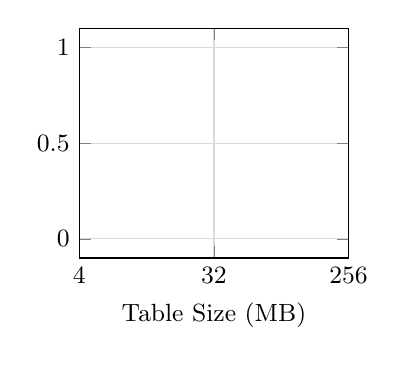
\begin{tikzpicture}
      \begin{axis}[
        width=5cm,
        height=4.5cm,
        xlabel={Table Size (MB)},
        % ylabel={Throughput (M/s)},
        xmode=log,
        log basis x=2,
        xmin=131072,
        xmax=268435456,
        xtick={262144,2097152,16777216,134217728},
        xticklabels={4,32,256,2048},
        grid=major,
        grid style={gray!30},
        tick label style={font=\small},
        label style={font=\small},
        scaled ticks=true,
        tick label style={/pgf/number format/fixed,/pgf/number format/precision=1}
      ]
      \AddAllObjectsForDataSize{6}
      \end{axis}
    \end{tikzpicture}
    \caption{\getScalingCaseName{6}}
  \end{subfigure}%
  % Case 7
  \begin{subfigure}[b]{0.24\textwidth}
    \tiny
    \centering
    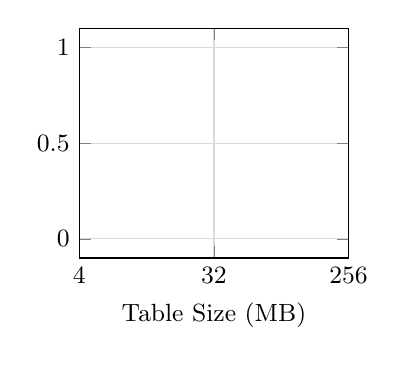
\begin{tikzpicture}
      \begin{axis}[
        width=5cm,
        height=4.5cm,
        xlabel={Table Size (MB)},
        % ylabel={Throughput (M/s)},
        xmode=log,
        log basis x=2,
        xmin=131072,
        xmax=268435456,
        xtick={262144,2097152,16777216,134217728},
        xticklabels={4,32,256,2048},
        grid=major,
        grid style={gray!30},
        tick label style={font=\small},
        label style={font=\small},
        scaled ticks=true,
        tick label style={/pgf/number format/fixed,/pgf/number format/precision=1}
      ]
      \AddAllObjectsForDataSize{7}
      \end{axis}
    \end{tikzpicture}
    \caption{\getScalingCaseName{7}}
  \end{subfigure}%
  \caption{Throughput vs Table Size (log-x) across operations. Styles match prior figures.}
  \label{fig:data_size_scaling}
\end{figure*}

% Include percentile tables
\begin{table*}[h!]
    \centering
    \footnotesize
    \caption{Latency Percentiles for Insertion and Positive Query Operations}
    \label{tab:latency_percentiles}
    \begin{tabular}{|c|ccccc|ccccc|}
        \toprule
        & \multicolumn{5}{c|}{Insertion} & \multicolumn{5}{c|}{Positive Query} \\
        \cmidrule(lr){2-6} \cmidrule(lr){7-11}
        Percentile & \htthree & \htfour & \htfive & \htone & \httwo & \htthree & \htfour & \htfive & \htone & \httwo \\
        \midrule
        $50.0\%$ & 226ns & 321ns & 452ns & 331ns & 172ns & 122ns & 236ns & 149ns & 283ns & 162ns \\
        $95.0\%$ & 1.5$\mu$s & 667ns & 34.3$\mu$s & 621ns & 349ns & 187ns & 489ns & 483ns & 560ns & 249ns \\
        $99.0\%$ & 4.3$\mu$s & 909ns & 61.4$\mu$s & 805ns & 539ns & 386ns & 651ns & 791ns & 731ns & 510ns \\
        $99.9\%$ & 13.7$\mu$s & 16.5$\mu$s & 104$\mu$s & 1.1$\mu$s & 715ns & 1.1$\mu$s & 889ns & 1.3$\mu$s & 1.0$\mu$s & 592ns \\
        $99.99\%$ & 162$\mu$s & 18.6$\mu$s & 291$\mu$s & 3.8$\mu$s & 1.1$\mu$s & 162$\mu$s & 3.5$\mu$s & 2.0$\mu$s & 3.6$\mu$s & 736ns \\
        max & 0.79s & 0.18s & 40.8ms & 106ms & 0.14s & 0.79s & 293$\mu$s & 306$\mu$s & 286$\mu$s & 277$\mu$s \\
        \bottomrule
    \end{tabular}
\end{table*}



\end{document}
